\documentclass[conference]{IEEEtran}
\usepackage[T1]{fontenc}
\usepackage{graphicx}
\usepackage{booktabs}
\usepackage{amsmath}
\usepackage{url}
\usepackage{tikz}
\usetikzlibrary{arrows.meta,positioning}
\usepackage[colorlinks=true,allcolors=blue!55!black]{hyperref}
\hypersetup{
  pdftitle={Geometry-First Generative Worlds as Simulation Substrates in Bronchoscopy},
  pdfauthor={Chris von Csefalvay; Pranav Doma; Tamas Foldi},
  pdfsubject={SynAirG: geometry-first bronchoscopy simulation},
  pdfkeywords={SynAirG, bronchoscopy, synthetic data, surgical simulation, SLAM}
}
% auto-generated by spark_stats.py, do not edit by hand
\newcommand{\DSepisodes}{1000}
\newcommand{\DSframestotal}{1\,769\,286}
\newcommand{\DShours}{24.6}
\newcommand{\DSfps}{20}
\newcommand{\DSdurmed}{91}
\newcommand{\DSbranchmed}{170}
\newcommand{\DSgenmed}{17}
\newcommand{\DStermmed}{87}
\newcommand{\DScenterlinemed}{238}
\newcommand{\DSairwaymlmed}{46}
\newcommand{\DSpathmed}{743}
\newcommand{\DSlumenmed}{3.3}
\newcommand{\DSspeedmed}{8}
\newcommand{\DSangmed}{4}
\newcommand{\DSinsertmed}{234}
\newcommand{\DSpassrate}{100.0}
\newcommand{\DScasessampled}{33}
\newcommand{\DSparquetsampled}{33}
\newcommand{\DSdistinctN}{33}
\newcommand{\DSdistinctfrom}{50}
\newcommand{\DSbranchlo}{116}
\newcommand{\DSbranchhi}{359}
\newcommand{\DSgenlo}{9}
\newcommand{\DSgenhi}{36}
\newcommand{\DSclmin}{1.7}
\newcommand{\DSclmax}{4.7}
\newcommand{\DSuniqueworlds}{56}
\newcommand{\DSdupepisodes}{941}
\newcommand{\DSmaxmult}{29}

\setlength{\textfloatsep}{6pt plus 1pt minus 2pt}
\setlength{\floatsep}{5pt plus 1pt minus 1pt}
\setlength{\abovecaptionskip}{4pt}

\newcommand{\synairg}{\textsc{SynAirG}}

\begin{document}

\title{Geometry-First Generative Worlds as\\Simulation Substrates in Bronchoscopy}

\author{\IEEEauthorblockN{Chris von Csefalvay, Pranav Doma and Tamas Foldi}
\IEEEauthorblockA{HCLTech\\
Correspondence: \href{mailto:kristof.csefalvay@hcltech.com}{kristof.csefalvay@hcltech.com}}}

\maketitle

\begin{abstract}
The limiting factor for endoluminal robotics in bronchoscopic approaches is not algorithms but supervision -- essentially, a data problem: recordings are scarce, privacy-encumbered and rarely carry ground truth for pose nor depth. We describe \synairg{}, a manifest-driven procedural pipeline that turns chest CTs into navigable, metric bronchoscopy worlds. In the generative setting, procedurally synthesised volumes are reduced to quality-assured airway meshes and centreline graphs, procedure-style scope trajectories are sampled, and frame-aligned depth, surface normals and per-pixel shading streams are rendered with exact pose. All of this is packaged in the LeRobot and TUM trajectory formats, ready for SLAM training or other downstream applications. We validate the methodology on a large set of synthetic cases, characterising anatomical and kinematic spread. We then report pitfalls with equal candour, including how corpus-level fingerprinting of the full release exposed silent anatomical mode collapse caused by cache reuse upstream of otherwise-passing per-case quality gates, and we outline two unaddressed realism gaps, conditional neural appearance for mucosal pathology and prescribed respiratory deformation, with concrete pathways for both. Geometry-first generation reconciles the desire for realism with the need for customisability and cross-temporal stability.
\end{abstract}

\section{Introduction}
Autonomy in bronchoscopy, whether assistive localisation, closed-loop navigation or interventional planning (with or without adjunctive methods like radiographic navigation, EM localisation or EBUS) is starved of training signal. Patient recordings are scarce and privacy-encumbered, and even where video exists it carries no pose, no depth and no per-voxel geometry against which perception can be supervised or evaluated. Phantom and cadaver studies provide geometry but not anatomical variation, patient-specific virtual bronchoscopy \cite{kiraly2004} requires a CT per subject and inherits the same scarcity and privacy aspects alike. The airway analysis community have produced excellent segmentation benchmarks \cite{lo2012exact,zhang2023atm,stoverud2024aeropath}, but these are primarily volumetric label sets, not navigable worlds with episodes, trajectories and rendered observations. Reinforcement learning needs more.

The currently fashionable response is to generate appearance directly, leveraging video diffusion models that dream plausible endoscopic scenes \cite{li2024endora}. These produce convincing pixels but no metric backbone. There is no reusable pose, no consistent geometry across frames, no anatomy that can be interrogated, deformed or re-rendered, and therefore nothing against which standard odometry or depth metrics \cite{sturm2012tum,eigen2014depth} can be computed.

We argue for the inverse ordering: \emph{synthesise the patient} (geometry first), \emph{not the pixels} (appearance later). We draw on MAISI,\cite{zhao2026maisiv2} a generative CT model to supply population-scale anatomy. A deterministic procedural pipeline then reduces each volume to a navigable airway world with exact meshes, centrelines and camera trajectories. Finally, rendering then emits geometry-anchored observation streams. Appearance thus becomes a swappable conditional layer on top of (i.e. conditioned by) a durable metric ground truth, so that sim-to-real transfer \cite{tobin2017domain} becomes a rendering-domain problem rather than a data problem. Every appearance variant thus inherits geometry grounded supervision for free. This is the substrate layer that digital-twin framings of surgical data science presuppose \cite{ding2024digital}.

This paper seeks to make four contributions. First, we describe \synairg{}, a manifest-driven pipeline from generative (or imported) thoracic CT to quality-gated bronchoscopy worlds. Second, we validate the methodology on a large set of verified-distinct cases drawn from a public dataset we share, with anatomical and kinematic characterisation. Third, we report our quality assurance practices and a cautionary finding from auditing that same instantiation at corpus level: per-case quality gates passed uniformly but an upstream caching defect silently collapsed anatomical diversity. This failure mode has been evidenced in other synthetic data sets, and we hope our cautionary tale may prevent similar collapse. Fourth, we outline the two realism gaps the pipeline intentionally omits: mucosal appearance and respiratory deformation, with concrete technical pathways for each.

\section{Related work}
Endoscopic datasets with geometric ground truth exist for the colon, where C3VD \cite{bobrow2023c3vd} registers real video to known phantom geometry, and EndoSLAM \cite{ozyoruk2021endoslam} provides ex-vivo trajectories; nothing comparable exists at scale for airways. Bronchoscopic localisation work has therefore leaned on patient-specific renders and small clinical sets \cite{visentini2017deep,shen2019context}. Generative imaging in radiography has matured to the point where latent diffusion models can reliably synthesise full CT volumes with paired anatomical labels \cite{guo2024maisi}. Typically, appearance is addressed using ControlNet-style conditional image generation \cite{zhang2023controlnet} and diffusion \cite{li2024endora}. \synairg{} occupies the gap between these realms: it consumes generative volumes and emits worlds ready for robot learning, leaving appearance as a downstream conditional stage.

\section{The \synairg{} pipeline}
\synairg{} is organised around a manifest-first 'bakery': every case is fully specified by a YAML or JSON 'recipe' (manifest) processed by a CLI, and every artefact carries provenance metadata sufficient to regenerate or audit it. Fig.~\ref{fig:pipeline} summarises the six stages.

\begin{figure}[t]
\centering
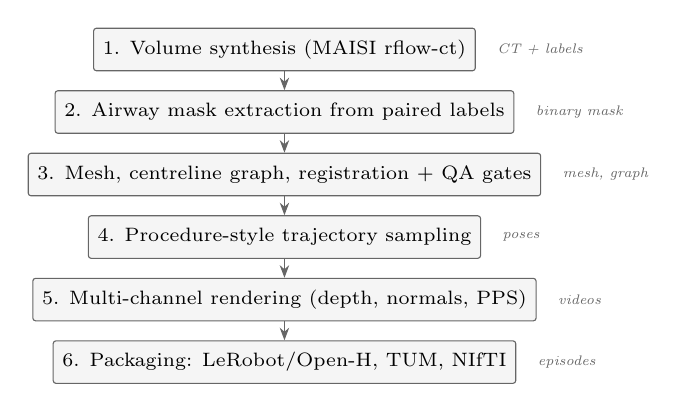
\begin{tikzpicture}[
  node distance=2.4mm,
  stage/.style={draw=black!60, rounded corners=1pt, fill=black!4,
    minimum width=46mm, minimum height=5.4mm, font=\scriptsize, align=center},
  art/.style={font=\tiny\itshape, text=black!60, align=left},
  arr/.style={-{Stealth[length=1.6mm]}, black!60}
]
\node[stage] (s1) {1. Volume synthesis (MAISI rflow-ct)};
\node[stage, below=of s1] (s2) {2. Airway mask extraction from paired labels};
\node[stage, below=of s2] (s3) {3. Mesh, centreline graph, registration + QA gates};
\node[stage, below=of s3] (s4) {4. Procedure-style trajectory sampling};
\node[stage, below=of s4] (s5) {5. Multi-channel rendering (depth, normals, PPS)};
\node[stage, below=of s5] (s6) {6. Packaging: LeRobot/Open-H, TUM, NIfTI};
\foreach \a/\b in {s1/s2,s2/s3,s3/s4,s4/s5,s5/s6} \draw[arr] (\a) -- (\b);
\node[art, right=1.5mm of s1] {CT + labels};
\node[art, right=1.5mm of s2] {binary mask};
\node[art, right=1.5mm of s3] {mesh, graph};
\node[art, right=1.5mm of s4] {poses};
\node[art, right=1.5mm of s5] {videos};
\node[art, right=1.5mm of s6] {episodes};
\end{tikzpicture}
\caption{The \synairg{} stages. Each stage is manifest-driven and independently invocable, and artefacts carry provenance for regeneration and audit.}
\label{fig:pipeline}
\end{figure}

\subsubsection*{Volume synthesis (for generative applications)} A wrapper around MAISI \cite{guo2024maisi} emits a chest CT and a paired multi-organ label map (512$\times$512$\times$256 voxels at 0.75$\times$0.75$\times$1.22\,mm in the instantiation below), requesting trachea, airway, lung lobes and heart. \synairg{} was primarily designed for SLAM training, and for this reason, is a non-pathological dataset. However, MAISI can synthesise a range of CT-visible peribronchial pathologies, and their integration is architecturally supported (indeed, it is core to the pathological set).

\begin{figure*}[t]
\centering
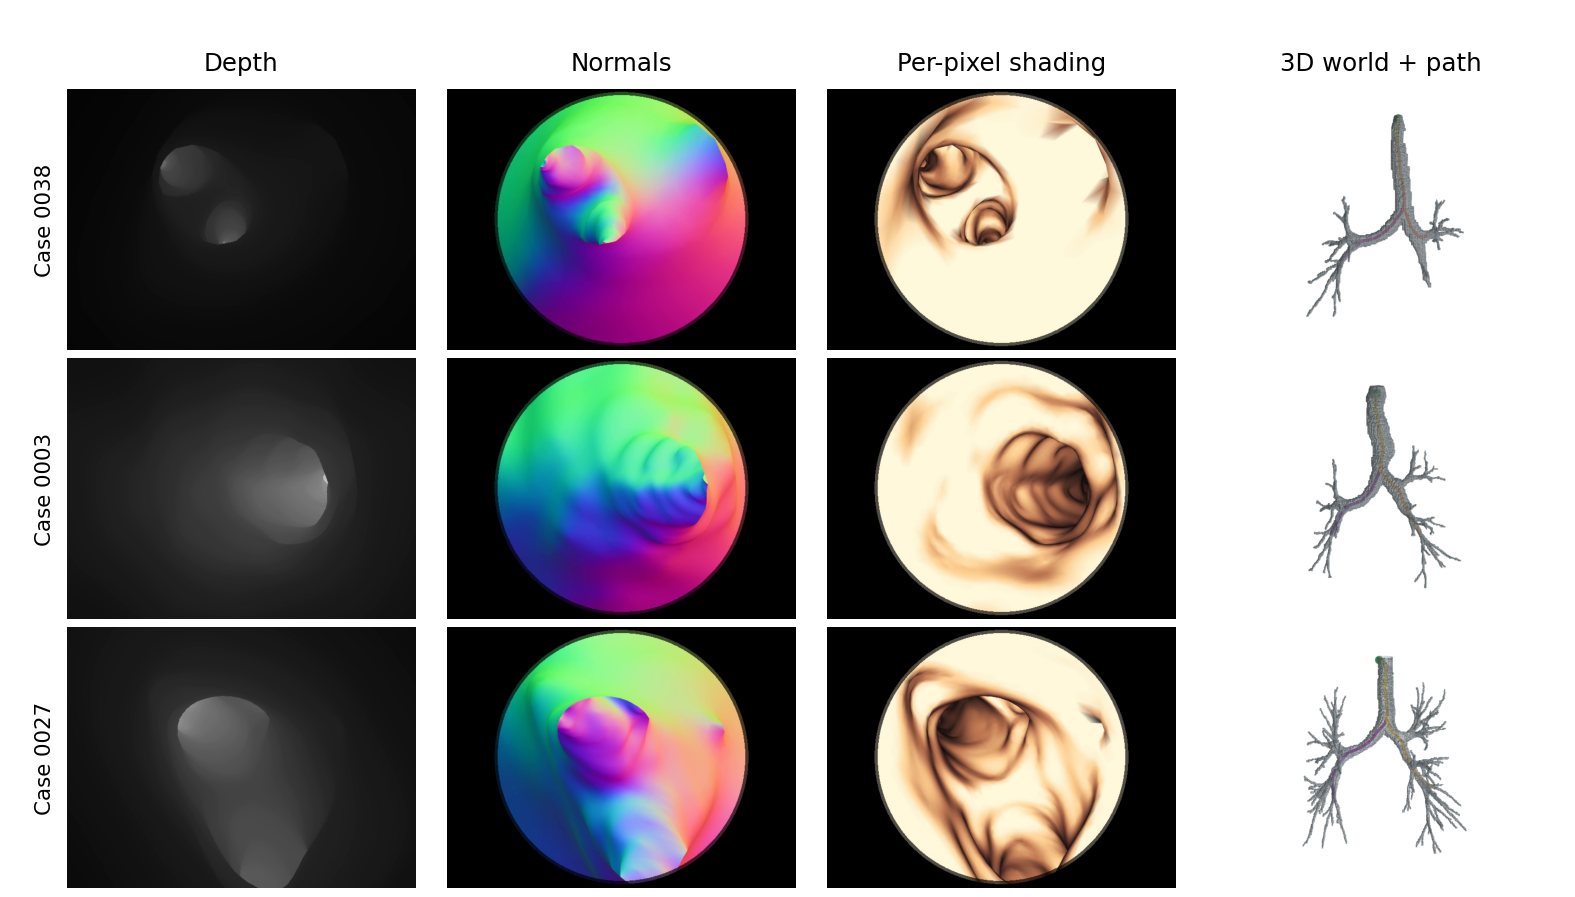
\includegraphics[width=0.92\textwidth]{figures/fig_montage.png}
\caption{Three distinct worlds from the working set (rows: shortest, median and longest centreline), frame-aligned depth, surface normals and per-pixel shading, with the reconstructed luminal surface and time-coloured procedure trajectory (rightmost). Every pixel is anchored to exact mesh geometry and scope pose.}
\label{fig:montage}
\end{figure*}

\subsubsection*{Mask extraction} The binary airway mask is taken from the generated label map rather than re-segmented, preserving generator-consistent topology. Small disconnected components are bridged or discarded under distance thresholds recorded in metadata.

\subsubsection*{Mesh and centreline} Marching cubes over the repaired mask yields a hollow, inward-oriented luminal mesh, which is then Taubin-smoothed, healed to a single connected component and trimmed to a single proximal opening. A skeleton graph provides the centreline with per-node radii, branch labels, generation depth and root-reachability. The mesh coordinates are mapped to the CT volumes through the registration rail.

\subsubsection*{Quality gates} Cases are accepted only if configurable per-case gates pass: minimum airway voxel count, minimum centreline nodes, minimum mesh vertices, full root reachability, expected proximal opening, no non-manifold edges or degenerate faces, and minimum procedure length and frame count. Rejections are logged with machine-readable reasons. In the released instantiation below, all released cases passed all gates.

\subsubsection*{Trajectory sampling} A multi-target procedure sampler selects reachable peripheral targets on the centreline graph and generates insertion and retraction phases with bounded curvature and lumen-aware clearance, mimicking the exploratory structure of diagnostic bronchoscopy rather than a single fly-through. The sampler is deliberately replaceable: the released trajectories are worked examples, the durable product is the geometry, and physically richer rollouts, e.g.\ Cosserat rod models of scope mechanics with lumen contact \cite{rucker2011}, can be driven over the same worlds without touching any upstream stage.

\subsubsection*{Rendering and packaging} A calibrated pinhole scope renders frame-aligned depth, surface normals and per-pixel shading (PPS) streams along the trajectory. Episodes are written in the LeRobot v2.1 layout \cite{cadene2024lerobot} with an 8-DoF action channel, TUM-format pose files \cite{sturm2012tum} for drop-in odometry evaluation, and per-case medical metadata including the full QA record. This is aligned with the Open-H \cite{openh2026embodiment} convention of LeRobot v2.1, \cite{cadene2024lerobot} and is easily importable into robotic training frameworks.



\section{Instantiation and characterisation}
We validate the pipeline on the public 1000lungs instantiation.\footnote{Dataset: \href{https://doi.org/10.57967/hf/9209}{doi:10.57967/hf/9209}. Code and viewer: \url{https://hcltech-robotics.github.io/synairg/}.} The release comprises \DSepisodes{} episodes totalling \DSframestotal{} frames (\DShours{}\,h at \DSfps{}\,fps, 640$\times$480), each bundling CT, labels, mask, mesh, centreline, scope path, three rendered condition streams and pose. RGB output is not a primary output modality, as it primarily pertains to appearance and thus deliberately treated as a different layer (Sec.~\ref{sec:appearance}). The release ships with an interactive episode viewer that streams the condition videos alongside live pose telemetry, phase state and bronchial-tree localisation.

Fig.~\ref{fig:montage} shows three of these worlds across the rendered modalities, and summary characteristics are described in Fig.~\ref{fig:char} and Table~\ref{tab:stats} characterise the set. This highlights the substantial diversity of generative worlds obtained without opinionated prompting (i.e. 'out of the box'): the anatomical spread is substantial, with branch counts that span \DSbranchlo--\DSbranchhi{}, maximum generation depth \DSgenlo--\DSgenhi{}, and total centreline length \DSclmin--\DSclmax\,m. These are broadly in line with classical morphometric expectations \cite{weibel1963}. Trajectories are intended to recapitulate procedural reality, with median tip speed of \DSspeedmed\,mm/s at median angular rate \DSangmed$^\circ$/s over a median \DSpathmed\,mm path visiting multiple peripheral targets per episode. \synairg{}'s localisation objective meant we opted to forgo any particular established methodology (e.g. Four Landmarks \cite{cold2023systematic}), but the procedural path generator can be adapted to any arbitrary imaging algorithm in a few lines.

\begin{figure*}[t]
\centering
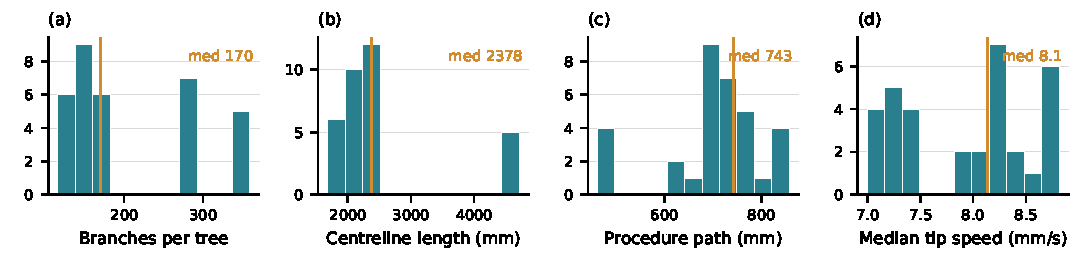
\includegraphics[width=0.94\textwidth]{figures/fig_characterisation.pdf}
\caption{Characterisation of a \DSdistinctN{}-sample set of verified distinct worlds: (a) branches per tree, (b) total centreline length, (c) procedure path length, (d) median tip speed (kinematics from the released 8-DoF action channel). Orange line: median.}
\label{fig:char}
\end{figure*}

\begin{table}[t]
\caption{Median characteristics of generated worlds.}
\label{tab:stats}
\centering
\begin{tabular}{@{}ll@{}}
\toprule
Episode duration & \DSdurmed\,s (\DSfps\,fps) \\
Branches per tree & \DSbranchmed{} (range \DSbranchlo--\DSbranchhi) \\
Maximum generation depth & \DSgenmed{} (range \DSgenlo--\DSgenhi) \\
Terminal branches & \DStermmed \\
Total centreline length & \DScenterlinemed\,cm \\
Airway luminal volume (pruned) & \DSairwaymlmed\,mL \\
Procedure path length & \DSpathmed\,mm \\
Minimum luminal diameter & \DSlumenmed\,mm \\
Median tip speed / angular rate & \DSspeedmed\,mm/s / \DSangmed$^\circ$/s \\
Max insertion depth & \DSinsertmed\,mm \\
\bottomrule
\end{tabular}
\end{table}

Because pose and depth are exact by construction, standard evaluation applies without annotation: absolute trajectory and relative pose error for odometry and SLAM \cite{sturm2012tum}, AbsRel and threshold accuracy for depth \cite{eigen2014depth}, and branch-level relocalisation against centreline labels.

\section{Pitfalls and open problems}
\label{sec:pitfalls}
\subsection{Replication and contamination}
Our experience highlighted an interesting pitfall that anyone generating training worlds may find an instructive failure. On our initial generation of a large number (several hundred) worlds, corpus-level fingerprinting of the full release revealed that several worlds ended up drawing on the same cached source material. Traditional workflows often focus on intra-sample, not inter-sample, consistency. This may allow duplicates and co-conditioned outputs to pass individual quality gates, e.g. in the case of seed collisions or cached reuses of generated or loaded CT volumes. The consequences of shipping such a corpus unaudited are serious: train/test splits leak, apparent generalisation becomes memorisation and benchmark numbers inflate silently.

Two remedies follow. Mechanically, per-case seeds should be threaded through every stochastic stage and every cache must be keyed on them. Structurally, quality assurance must include \emph{corpus-level} gates: the minimum is a uniqueness gate on the anatomy-trajectory fingerprint at generation time, and a published fingerprint manifest so downstream users can verify diversity and construct leakage-free splits. \synairg{}'s data collection schema has been designed to make this cheap: because \synairg{} metadata is geometry-first, fingerprinting this entire corpus, and every number in this paper, required roughly 30\,MB of transfer via column-projected and range reads.

\subsection{Appearance and pathology}
\label{sec:appearance}
The rendered streams are geometric by intent: mucosal appearance, and in particular pathology such as inflammation, erythema or secretions, are not modelled. The pipeline's design anticipates a neural texturing pathway we have deliberately not exercised for the initial release. The intent behind this is to preserve generalisation and allow downstream environments to parametrise such seed geometries as needed. This is in line with our selection of outputs: depth, normal and PPS buffers are exactly the multimodal control stack consumed by conditional diffusion \cite{zhang2023controlnet} and, notably, by world foundation models with transfer modes such as Cosmos \cite{nvidia2025cosmos}. Appearance-space generators are thus complements (typically, teachers of transfer models) rather than substitutes: our substrate provides spatiotemporally consistent geometry over which any renderer, parametrised by a text or label channel injecting pathology, can be clad. Cross-frame attention or mesh-anchored appearance (U,V-space textures or Gaussian primitives on the lumen \cite{kerbl20233dgs}) then enforce non-geometry temporal and viewpoint consistency. Under either variant the pose and depth ground truth is untouched: pathology becomes a controllable appearance axis benefiting from the guarantee of consistency a fixed metric world can afford.

\subsection{Respiratory deformation}
At present, the publicly released worlds are rigid, which real airways are of course not. A feasible solution is to drive the centreline graph and mesh with a reduced-order cage or skeleton-based deformation field whose amplitude grows with generation depth to mimic parenchymal tethering, phase coupled to a respiratory signal (whether deterministic or 4D-CT derived \cite{keall2006respiratory}). Because the deformation is known at every frame, the result continues to serve as a useful ground truth. Established soft-tissue frameworks \cite{faure2012sofa} or GPU-resident XPBD then integrate bronchoscope contact forces.

\section{Conclusion}
Geometry-first procedural generation turns generative CT into metric, navigable bronchoscopy worlds that offer exact supervision for reinforcement learning and sim-to-real transfer. Our own instantiation supplied both the validation and the cautionary tale: per-case quality assurance is not corpus quality assurance, and generative-world pipelines should ship fingerprint manifests and uniqueness gates as a matter of course. The code is released under Apache-2.0 and the 1000lungs dataset under OpenMDW 1.1, while an interventional (EBUS-guided TBNA) specific version is in preparation.

\bibliographystyle{SynAirGIEEEtran}
\bibliography{references}

\end{document}
